\documentclass{mc2015}

%%%%%%%%%%%%%%%%%%%%%%%%%%%%%%%%%%%%%%%%%%%%%%%%%%%%%%%%%%%%%%%%%%%%%
\usepackage[T1]{fontenc}         % Use T1 encoding instead of OT1
\usepackage[utf8]{inputenc}      % Use UTF8 input encoding
\usepackage{microtype}           % Improve typography
\usepackage{booktabs}            % Publication quality tables
\usepackage{amsmath}
\usepackage{mhchem}
\usepackage{graphicx}
\usepackage{gensymb}
\usepackage{float}
\usepackage{subcaption}
\usepackage[exponent-product=\cdot]{siunitx}
\usepackage[colorlinks,breaklinks]{hyperref}
\hypersetup{linkcolor=black, citecolor=black, urlcolor=black}

\usepackage{lipsum}

\def\equationautorefname{Eq.}
\def\figureautorefname{Fig.}

%%%%%%%%%%%%%%%%%%%%%%%%%%%%%%%%%%%%%%%%%%%%%%%%%%%%%%%%%%%%%%%%%%%%%
% Insert authors' names and short version of title in lines below

\authorHead{Madicken Munk, Leah Morgan, Brett Davidheiser-Kroll, et. al.}
\shortTitle{Design of a Compact Neutron Source for Geochronology Applications}

%%%%%%%%%%%%%%%%%%%%%%%%%%%%%%%%%%%%%%%%%%%%%%%%%%%%%%%%%%%%%%%%%%%%%
\begin{document}

\title{Design and Feasibility Study of a Compact Neutron Source for Extra-terrestrial Geochronology Applications}

\author{Madicken Munk}
\author{Rachel Slaybaugh}
\author{Karl Van Bibber}
\affil{Department of Nuclear Engineering \\
  University of California, Berkeley
  3115B Etcheverry Hall, Berkeley, CA \\
  madicken@berkeley.edu}

\author{Leah Morgan}
\author{Brett Davidheiser-Kroll}
\author{Darren Mark}
\author{Sanjeev Gupta}
\author{Patrick Harkness}
\affil{
  Scottish Universities Environmental Research Centre \\
  Rankine Avenue, East Kilbride G75 0QF, UK \\
  leah.morgan@glasgow.ac.uk
}

\maketitle

\begin{abstract}
The \ce{^{40}Ar}/\ce{^{39}Ar} radiometric dating technique is an attractive option for future martian age-dating applications. However, in-situ \ce{^{40}Ar}/\ce{^{39}Ar} radiometric dating on Mars presents unique challenges to the design of a device capable of achieving sufficient precision on geological samples obtained on the Martian surface. For this application, a fast neutron source with a low thermal neutron flux is ideal for inducing the \ce{^{39}K}(n,p)\ce{^{39}Ar} reaction with few competing reactions that require age-correction factors. This paper explores the design of a neutron emitting device specifically for in-situ geochronological applications on Mars. We have determined that the most feasible design is likely a \ce{^{252}Cf} spontaneous fission source shielded with layered polyethylene and a strong thermal neutron absorber. Although boosting options--induced fission sources, ($\alpha$,n)--are available, they do not provide sufficient neutron multiplicity to justify the increased mass of the device. Furthermore, shielding the rover from the neutron source will likely comprise the largest fractional mass of the device, which will be reduced by shielding only a fractional solid angle of the source. While we have determined that it is possible to design such a neutron source, there will also be other instrumentation competing for a mass fraction of the Rover instrument payload. The addition of this instrumentation may make it difficult to design a device that achieves the required mass and fluence limitations for a future mission.   

\emph{Key Words}: Fisson Sources, argon/argon Geochronology, Mars
\end{abstract}

%%%%%%%%%%%%%%%%%%%%%%%%%%%%%%%%%%%%%%%%%%%%%%%%%%%%%%%%%%%%%%%%%%%%%
\section{Introduction}

One of the goals of the future rover missions includes determining the age of Mars. Current efforts on this front have been focused on using the \ce{^{40}K}/\ce{^{40}Ar} method (henceforth referred to as the K/Ar method) \cite{farley_situ_2014,farley_double-spike_2013,cassata_situ_2014}. This method relies upon the fact that \ce{^{40}K} decays to \ce{^{40}Ar}. Assuming that at the time of formation there is no argon in the sample (a good assumption, as the gas thermodynamically driven to diffuse out of the molten rock), an age can be calculated with this parent-daughter ratio \cite{mcdougall_geochronology_1999}. This method is not without its drawbacks though. To count the relative abundances of \ce{^{40}K} and \ce{^{40}Ar}, separate processes are required to isolate each element, so two samples are required. Additionally, the abundance counts for each element are an average across each crystal.
%crystal?
 If the sample has a complex thermal history, the gaseous argon is likely to have diffused to the crystal boundaries during each thermal event, which can skew the age.  

McDougall \cite{mcdougall_geochronology_1999}\\
Farley age of Mars \cite{farley_situ_2014}\\
Farley K-Ar description for rover \cite{farley_double-spike_2013}\\
Li paper on lunar sources \cite{li_evaluation_2011}\\
Cassata \cite{cassata_situ_2014}

Need to briefly describe ar-ar  method before you talk about why it's attractive.

The \ce{^{40}Ar}/\ce{^{39}Ar} method for evaluating the age of geological samples is attractive for a number of reasons: (1) it reveals information about the thermal history of the sample, (2) potassium is readily abundant in much of the Martian surface, so acceptable counting statistics are achievable on many potential samples, and (3) it is a well-understood method with a large experience base. 

The remainder of this paper will discuss ... Section \ref{sec:design} covers the details of the device design. The feasibility of device configurations is discussed in Section \ref{sec:feasibility}, and future work in Section \ref{sec:future}. Finally, concluding remarks are made in Section \ref{sec:conclusions}.

%%%%%%%%%%%%%%%%%%%%%%%%%%%%%%%%%%%%%%%%%%%%%%%%%%%%%%%%%%%%%%%%%%%%%
\section{Device Design}
\label{sec:design}

Add an introductory statement about what you need to achieve in the device design and why (list below). \\Next discuss a little bit about the approach and strategy (how did you get to the things in the picture?). \\ Describe what calculations you did.

[INCLUDE] flux requirements\\
temperature requirements\\
neutron energy limitations\\
competing reactions

A neutron emitting device that is optimized for in-situ irradiation and geochronological analysis will have a number of components. For the irradiation, a source producing a sufficiently high fast neutron flux

Complete device designs were simulated with MCNP5~\cite{brown_mcnp_2002}. Several geometries were considered (Fig. \ref{fig:geometries}). 

\begin{figure}[H]
  \centering
  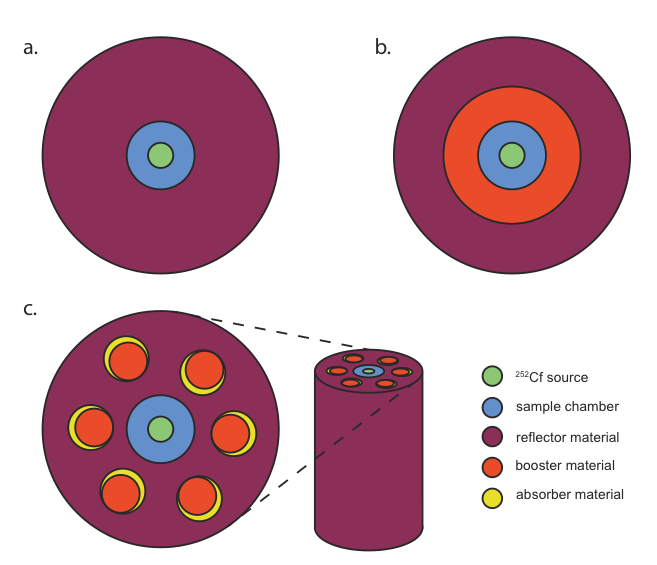
\includegraphics[width=0.5\textwidth]{Geometries.png}
  \caption{Configurations of devices for in-situ \ce{^{40}Ar}/\ce{^{39}Ar} geochronology. (a) A simple point source with a spherical shield/reflector, (b) a point source with spherical boosting material surrounded by a shield/reflector, (c) cylindrical assembly with centrally-located point source surrounded by boosting rods or rotatable boosting drums and shield/reflector.}
  \label{fig:geometries}
\end{figure}

The authors did not consider compact fusion sources, which have been considered for terrestrial \ce{^{40}Ar}/\ce{^{39}Ar} geochronology \cite{renne_application_2005}, as they are not mass-feasible for this application. Furthermore, we did not consider critical configurations of the device, as the device will be irradiating the sample for hundreds of days at a time and a system to compensate for reactivity feedback and other physical effects will add unnecessary complexity to an already inflexible design criteria. Transition sentence introducing the remainder of the section.


\subsection{Neutron Source}

A number of neutron source options were considered. Isotopes decaying by some probability of spontaneous fission offer a predictable neutron source flux with a sufficiently high quantity of fast neutrons. However, these sources also decay over time, so sample irradiation times will increase over the lifetime of the device to achieve the same fluence. Passive capture sources, like ($\alpha$,n) reactions, are attractive because two elements are required to create neutrons. This could mean source strength could be user-controlled, prolonging the life of the neutron source and, consequently, the entire device. Boosting material offers similar benefits to the latter and can be chosen to maximize fast neutron creation.   

\subsubsection{Passive fission sources}

Table \ref{tab:fisssource} compares the total mass and heat output for a number of different spontaneous fission isotopes (SF BR is spontaneous fission branch ratio). This was calculated with existing fission yield data in the literature~\cite{england_evaluation_1995, axton_neutron_1985}.
%This is illustrated in Table \ref{tab:fisssource}, which highlights the differences between many elements decaying by spontaneous fission. 
No isotope seems to completely satisfy all of the requirements of the passive fission sources.
% but you haven't told us what those are?
 Some have long half lives but require significant mass. Others create too much heat and will cause a premature release of natural and radiogenic argon. \ce{^{252}Cf} appears to most closely satisfy the heat output and mass requirements while also having a reasonably long half life. \ce{^{252}Cf} has the added benefit of broad user experience \cite{martin_production_2000} and a slightly faster neutron energy spectrum than that of \ce{^{235}U} \cite{hjalmar_energy_1955}. However, using \ce{^{252}Cf} as the sole neutron source in the device does pose some disadvantages: the device lifetime is unlikely to exceed the lifetime of the Mars rover as the half life is quite short, and it will take several years in a specialized reactor to produce enough \ce{^{252}Cf} to supply the source requirement desired for these purposes. 

For all MCNP5 simulations a source definition with a watt fission spectrum reflecting \ce{^{252}Cf} was used \cite[Appendix~C]{valentine_mcnp-dsp_1997}. 
% This sentence should go where you describe your calculations.

 \begin{table}
  \centering
  \caption{Passive neutron sources decaying by spontaneous fission}
  \begin{tabular}{l|ccccc}
    \toprule
    Source & Mass for $10^{11}$ $\frac{n}{sec}$ & $\frac{n}{sec-mg}$ & $t_{1/2}$ & SF BR (\%) & Heat Out ($\frac{Watts}{10^{11} source}$) \\
    \midrule
    \ce{^{252}Cf}& \num{43} mg & \num{2.3e9} & \num{2.645} years & \num{3.82} & \num{1.43} \\
    \ce{^{250}Cf} & \num{9.5} g & \num{1.1e10} & \num{13.08} years & \num{0.08} & \num{31}  \\
    \ce{^{248}Cm} & \num{2.1} kg & \num{4.7e10} & \num{3.5e5} years & \num{8.26} & \num{1.04}  \\
    \ce{^{246}Cm} & \num{9.8} kg & \num{1.0e10} & \num{4.7e3} years & \num{0.03} & \num{90}  \\
    \ce{^{244}Cm} & \num{9.8} kg & \num{1.0e10} & \num{18} years & \num{1.3e-4} & \num{2.4e4}  \\
    \ce{^{253}Es} & \num{274} g & \num{3.6e8} & \num{20} days & \num{8.7e-6} & \num{2.1e5}  \\
    \ce{^{254}Fm} & \num{0.2} mg & \num{5.0e11} & \num{3.24} hours & \num{0.06} & \num{33}  \\
	\bottomrule
  \end{tabular}
  \label{tab:fisssource}
\end{table}

\subsubsection{Passive capture sources}

Passive capture sources \cite{weise_neutron_1984,jacobs_energy_1983,marsh_high_1995} are those that generate neutrons by some capture reaction (excluding neutron capture, which is detailed in a subsequent section). Originally, these sources were attractive because separation of the element emitting the incident particle from the target would cease neutron production. % I am unsure about what this sentence means?
 The ability to "shut down" the neutron source would reduce the required neutron shielding for the Mars rover (assuming dose limits are fluence rather than dose rate dependent) and only require that the rover is constantly shielded from $\alpha$ particles.  Additionally, the neutron energy spectrum from this reaction is relatively fast. %However, these sources require homogenized mixing to supply the neutron flux defined previously.
However, the total neutron production is on the order of a few  neutrons per $10^6\:\alpha$ particles per second or less for most materials \cite{weise_neutron_1984,jacobs_energy_1983}. Consequently, for a $10^{11}$ neutron/s source, a roughly $10^{17}$ $\alpha$/s source would be required. 
% Why do we care about alphas? It seems like you're trying to argue that you would need too much mass - I think the alphas are distracting and you should talk more concretely about mass and half life. 
This is substantially more than the current $\alpha$ particle source rate from the RTG on Curiosity. Despite considering passive capture sources for in-situ \ce{^{40}Ar}/\ce{^{39}Ar} geochronology on lunar missions \cite{li_evaluation_2011}, a martian mission has significantly tighter mass and volume limitations. Therefore, while it is possible to obtain an alpha source that is large enough from an emission standpoint, the neutron source would either be of significant mass, which will violate mission limits, or with a short half-life, which will not meet time requirements.

\subsubsection{Boosting material}

The boosting material considered loosely falls into two categories: induced fission neutron sources, and neutron capture neutron sources. Both of these sources require an additional driving neutron source to produce neutrons. Induced fission sources can offer substantial multiplicitave boosting if the device configuration is near critical.  Much of the previous work on determining the minimum critical mass of induced-fission sources  was done with homogenized layers of fissionable material and moderator to enhance thermally-induced fission neutrons \cite{karni_semi-automated_keff,karni_smores_2003,goluoglu_smoresnew_2002}. This is not an attractive option for this application since a large fraction of the neutron flux will be thermal and thus unusable for the \ce{^{39}K}(n,p)\ce{^{39}Ar} reaction. Of the induced fission sources, blah blah blah were considered, as illustrated in Fig. \ref{fig:boosters}.

\begin{figure}[H]
  \centering
  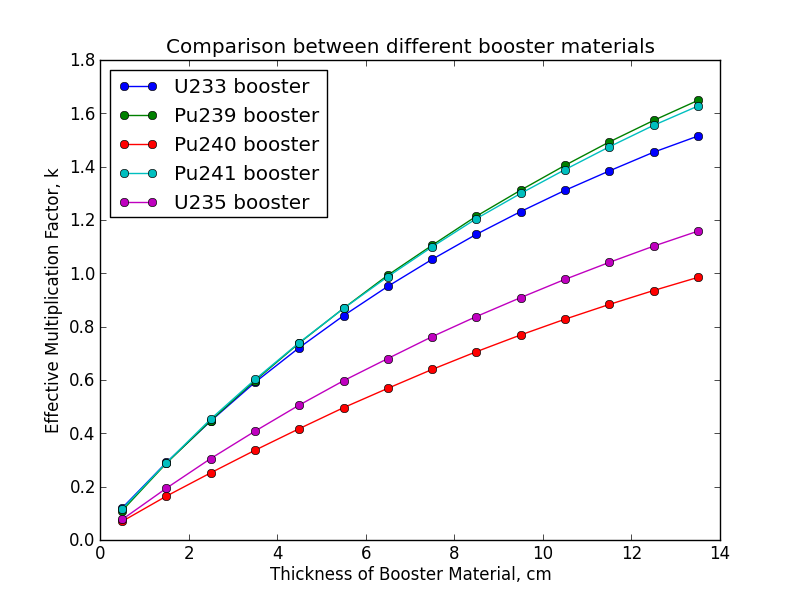
\includegraphics[width=4.5in]{Boosters.png}
  \caption{Induced fission neutron boosters}
  \label{fig:boosters}
\end{figure}

Of the neutron capture sources, the most attractive appeared to be the (n,2n) and (n,3n) fast neutron reactions in beryllium metal. A variant of Fig. \ref{fig:geometries} (?) was simulated with MCNP5, with a \ce{^{252}Cf} point source surrounded by a spherical shell of \ce{^{9}Be} metal, shielded with a premadex shell (what's that?).
To find the best design, the thickness of the \ce{^{9}Be} shell was varied; Fig. \ref{fig:beboosters} summarizes these results. As the thickness of \ce{^{9}Be} increases so does the flux boost, peaking at a $\sim$10\% boost with an 8.5cm shell around the point source. Although this boost is not negligible, it is not worth the added mass of $\sim$5.6kg, which would only offset a short increment of \ce{^{252}Cf} decay losses. %The beryllium may at first seem attractive as an ($\alpha$,n) source, but the flux boost from this reaction is several orders of magnitude less than the boosting from the (n,2n) and (n,3n) reactions, so it is not included.  
% I don't think you need the last sentence - if you want to keep it in reword since it's a little confusing

\begin{figure}[H]
  \centering
  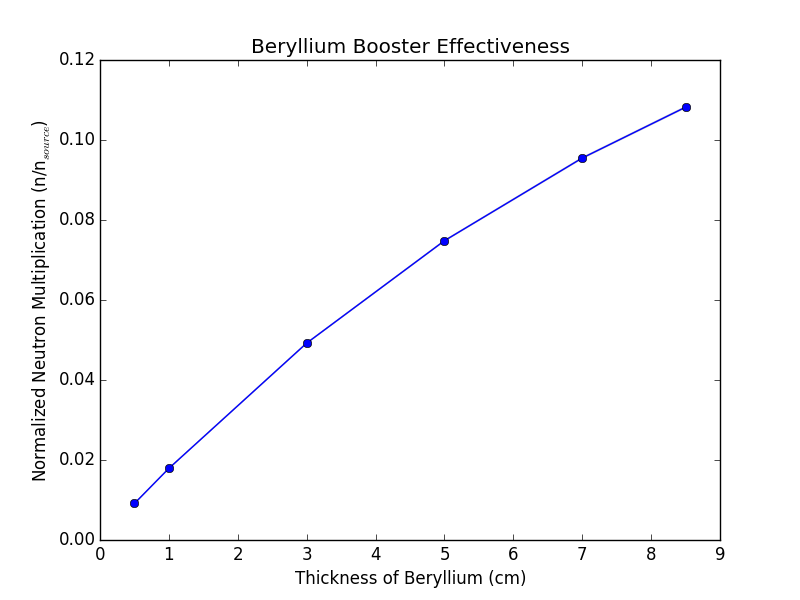
\includegraphics[width=4.5in]{Be_boost.png}
  \caption{Boosting the neutron flux with beryllium}
  \label{fig:beboosters}
\end{figure}

\subsection{Neutron Shield Design}

The most basic shield design is surrounding a point source of neutrons with a \ce{^{252}Cf} energy spectrum with a spherical shell of shield material. Figure \ref{fig:basics} illustrates the reduction in source strength as a function of radial distance away from the point source for a number of shield material options. Premadex is a hydrogenous material enriched in \ce{^{6}Li}. 

\begin{figure}[H]
  \centering
  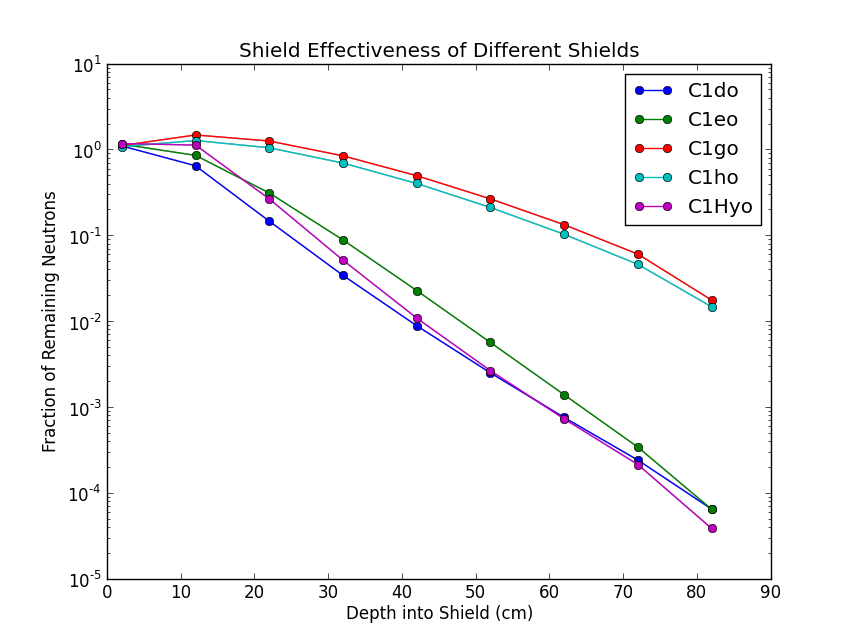
\includegraphics[width=4.5in]{Basics.png}
  \caption{Performance comparison for various shield material options}
  \label{fig:basics}
\end{figure}

A composite shield option designed to moderate and then absorb neutrons is likely the best option to reduce the radial thickness of required shield material. As illustrated in \ref{fig:basics}, the hydrogenous materials perform far better than the thermal neutron-absorbing metals, which should be expected as there is no moderator to maximize absorption in the latter. The thermal neutron absorbers, like Cd or Gd are well suited for neutron absorption of a predominantly thermal neutron energy spectrum.  fission spectrum of \ce{^{252}Cf} is moderated with a lighter atomic mass material and then a thin foil of Cd or Gd could be used to remove the peak thermal neutron flux. For polyethylene, Fig. \ref{fig:polychar} indicates that the maxiumum thermal neutron flux fraction occurs ~ 15-20cm away from the point source. For premadex this location is at ~12-15cm (\ref{fig:premchar}). However, the polyethylene has a much greater specific linear scattering efficiency, so foil placement could still be effective if placed before the peak thermal flux. 

\begin{figure}[H]
	\centering
	\begin{subfigure}{0.49\textwidth}
		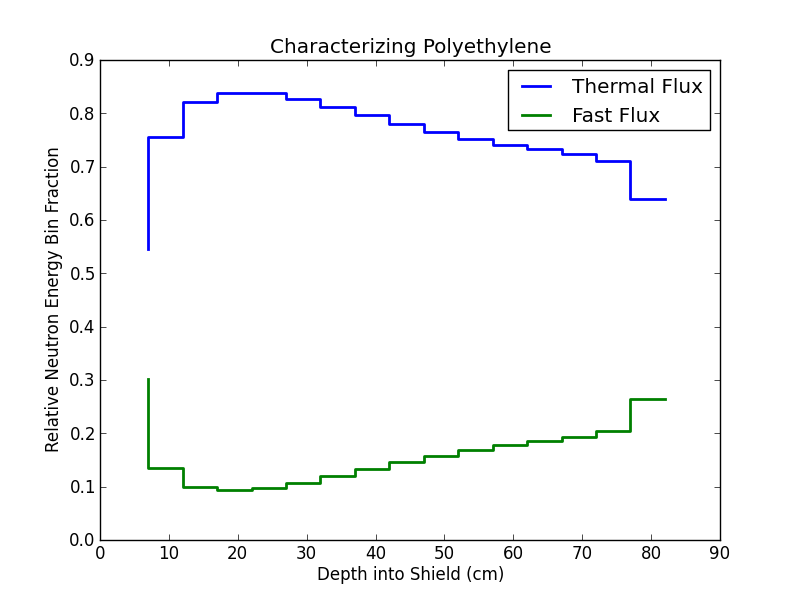
\includegraphics[width=\textwidth]{Poly_char.png}
		\caption{Polyethylene}
		\label{fig:polychar}
	\end{subfigure}
	\begin{subfigure}{0.49\textwidth}
		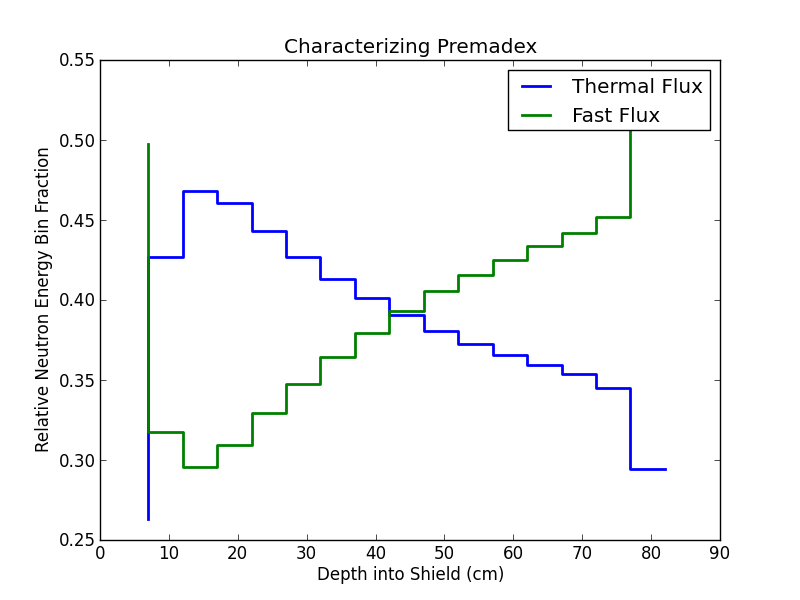
\includegraphics[width=\textwidth]{Prem_char.png}
		\caption{Premadex}
		\label{fig:premchar}
	\end{subfigure}
	\caption{Neutron Energy Spectra Comparison between thermalizing shield options. Thermal energies are below 0.1eV and fast energies are greater than 0.1MeV}
	\label{fig:chars}
\end{figure}

\subsection{Other Considerations}

A device optimized for the in-situ irradiation and age determination of geological samples requires an instrument payload in addition to the neutron emitting device. This will include, but is not limited to: a drilling mechanism, a mass spectrometer, and a system with which to heat up the sample to perform step-heating. 

%%%%%%%%%%%%%%%%%%%%%%%%%%%%%%%%%%%%%%%%%%%%%%%%%%%%%%%%%%%%%%%%%%%%%
\section{Feasibility of Device Configurations}
\label{sec:feasibility}

%%%%%%%%%%%%%%%%%%%%%%%%%%%%%%%%%%%%%%%%%%%%%%%%%%%%%%%%%%%%%%%%%%%%%
\section{Future Work}
\label{sec:future}

Thus far, the neutronic feasiblity of this device design has been explored. However, a number of other considerations must also be accounted for in greater detail in future analyses. Heat transfer calculations should be performed to ensure that the sample temperature will not exceed 200\celsius, which will lead to premature release of trapped argon in the sample. This calculation is contingent upon concrete knowledge of the design materials and geometry, and could be performed with some finite element heat transfer package. \\

Furthermore, selecting a power source to provide sufficient energy with which to step heat the sample to acceptable temperatures will be important. The most recent K/Ar age of Mars was heated to 890\celsius \cite{farley_situ_2014}, which does not reach the temperatures usually required for complete sample step heating, ~1200\celsius \cite{mcdougall_geochronology_1999}. Powering a device to heat the sample to this temperature may temporarily disable the rover or even exceed current design limitations. However, both the \ce{^{40}Ar}/\ce{^{39}Ar}  and \ce{^{40}K}/\ce{^{40}Ar}  age calculations may be skewed without adequate heating. \\

The shielding analysis and optimization detailed in this paper was exclusively for neutron shielding. Future rovers will also have photon dose limits, which will require shielding to ensure that the electronics do not degrade at an unacceptable rate. The addition of thermal neutron absorbers in a composite shield option, like Cd or Gd, will produce high energy photons that may have adverse effects on the overall damage rate of the device. 
Further optimization on the minimization of shield mass and volume will be beneficial to the overall device mass minimization. Should fissionable booster options be considered, it would also be ideal to minimize the boosting material mass to achieve a desired subcritical multiplication factor. Existing software to determine the minimize critical mass \cite{goluoglu_smoresnew_2002,karni_semi-automated_keff,karni_smores_2003} of systems and optimization of shield designs \cite{greenspan_material_1994,greenspan_swans:_2001} are available in the SCALE package \cite{bowman_scale_2003}. Utilization of this software in future design iterations would aid in the convergence to a realistic device design.  

%%%%%%%%%%%%%%%%%%%%%%%%%%%%%%%%%%%%%%%%%%%%%%%%%%%%%%%%%%%%%%%%%%%%%
\section{Conclusions}
\label{sec:conclusions}

A compact neutron source is an attractive candidate to induce the necessary reactions for  \ce{^{40}Ar}/\ce{^{39}Ar}  geochronological applications on future, unmanned, missions to extra-terrestrial bodies where sample return is neither feasible nor likely. However, the vast range of overall dose and dose rate limits for existing  rover designs lead to ambiguity in shielding designs, making optimization difficult. Furthermore, the longevity of the neutron source is likely to be compromised with the use of exclusively the 252Cf fission neutron source. This could be avoided with boosting material, but that would also require some moderation around all 4$\pi$ solid angles of the boosting material to achieve increased efficiency in neutron-induced fission. The addition of both shielding material and enough boosting material to achieve a high enough effective multiplication factor renders this configuration likely unfeasible. While the extent of this paper is dedicated to the analysis and design of a neutron source that can produce an acceptable fluence on reasonable timescales, the device designed for geochronological applications will include an additional instrument payload. These instruments, such as a mass spectrometer, can be optimized to have a greater abundance sensitivity. This could offset the loss of precision from a lower flux neutron source, but will undoubtedly come at a greater mass expense. Prioritizing which of these is more important will be imperative in moving forward with future designs. The total mass threshold could be increased if the RTG on the rover could be replaced with the neutron device. This would require a much more sophisticated heat removal and power conversion system than we have proposed for the device described in this paper. Furthermore, the need of a small neutron emitting device could be avoided if other space reactor concepts are considered for future missions to Mars. In this case, a system not unlike the setup at the Oregon State TRIGA reactor could be designed for sample irradiation. 

%%%%%%%%%%%%%%%%%%%%%%%%%%%%%%%%%%%%%%%%%%%%%%%%%%%%%%%%%%%%%%%%%%%%%
\section{Acknowledgments}

The primary authors would like to thank their collaborators for their wealth of knowledge and support on this project. In particular, we would like to thank the participants of our design review, held in Spring of 2014: Paul Renne, Tim Becker, Karl Van Bibber, Peter Hosemann, Max Fratoni, Rachel Slaybaugh, Richard Firestone, and Cory Waltz. We also would like to thank the European Space Agency for their generous financial support for this endeavor. Additionally, we thank Roger Scott, David Gilliam from NIST, David Thomas from NPL, and Ken Farley for their valuable advice and input on this project. 

%%%%%%%%%%%%%%%%%%%%%%%%%%%%%%%%%%%%%%%%%%%%%%%%%%%%%%%%%%%%%%%%%%%%%
\setlength{\baselineskip}{12pt}

\bibliographystyle{mc2015}
\bibliography{references}

%%%%%%%%%%%%%%%%%%%%%%%%%%%%%%%%%%%%%%%%%%%%%%%%%%%%%%%%%%%%%%%%%%%%%

\end{document}
